%% abtex2-modelo-artigo.tex, v-1.7.1 laurocesar
%% Copyright 2012-2013 by abnTeX2 group at http://abntex2.googlecode.com/ 
%%
%% This work may be distributed and/or modified under the
%% conditions of the LaTeX Project Public License, either version 1.3
%% of this license or (at your option) any later version.
%% The latest version of this license is in
%%   http://www.latex-project.org/lppl.txt
%% and version 1.3 or later is part of all distributions of LaTeX
%% version 2005/12/01 or later.
%%
%% This work has the LPPL maintenance status `maintained'.
%% 
%% The Current Maintainer of this work is the abnTeX2 team, led
%% by Lauro César Araujo. Further information are available on 
%% http://abntex2.googlecode.com/
%%
%% This work consists of the files abntex2-modelo-artigo.tex and
%% abntex2-modelo-references.bib
%%

% ------------------------------------------------------------------------
% ------------------------------------------------------------------------
% abnTeX2: Modelo de Artigo Acadêmico em conformidade com
% ABNT NBR 6022:2003: Informação e documentação - Artigo em publicação 
% periódica científica impressa - Apresentação
% ------------------------------------------------------------------------
% ------------------------------------------------------------------------

\documentclass[
	% -- opções da classe memoir --
	article,			% indica que é um artigo acadêmico
	11pt,				% tamanho da fonte
	oneside,			% para impressão apenas no verso. Oposto a twoside
	a4paper,			% tamanho do papel. 
	% -- opções da classe abntex2 --
	%chapter=TITLE,		% títulos de capítulos convertidos em letras maiúsculas
	%section=TITLE,		% títulos de seções convertidos em letras maiúsculas
	%subsection=TITLE,	% títulos de subseções convertidos em letras maiúsculas
	%subsubsection=TITLE % títulos de subsubseções convertidos em letras maiúsculas
	% -- opções do pacote babel --
	english,			% idioma adicional para hifenização
	brazil,				% o último idioma é o principal do documento
	]{abntex2}


% ---
% PACOTES
% ---

% ---
% Pacotes fundamentais 
% ---
\usepackage{amsmath}
\usepackage{cmap}				% Mapear caracteres especiais no PDF
\usepackage{lmodern}			% Usa a fonte Latin Modern
\usepackage[T1]{fontenc}		% Selecao de codigos de fonte.
\usepackage[utf8]{inputenc}		% Codificacao do documento (conversão automática dos acentos)
\usepackage{indentfirst}		% Indenta o primeiro parágrafo de cada seção.
\usepackage{nomencl} 			% Lista de simbolos
\usepackage{color}				% Controle das cores
\usepackage{graphicx}			% Inclusão de gráficos
% ---
		
% ---
% Pacotes adicionais, usados apenas no âmbito do Modelo Canônico do abnteX2
% ---
\usepackage{lipsum}				% para geração de dummy text
% ---
		
% ---
% Pacotes de citações
% ---
\usepackage[brazilian,hyperpageref]{backref}	 % Paginas com as citações na bibl
\usepackage[alf]{abntex2cite}	% Citações padrão ABNT
% ---

% ---
% Configurações do pacote backref
% Usado sem a opção hyperpageref de backref
\renewcommand{\backrefpagesname}{Citado na(s) página(s):~}
% Texto padrão antes do número das páginas
\renewcommand{\backref}{}
% Define os textos da citação
\renewcommand*{\backrefalt}[4]{
	\ifcase #1 %
		Nenhuma citação no texto.%
	\or
		Citado na página #2.%
	\else
		Citado #1 vezes nas páginas #2.%
	\fi}%
% ---

% ---
% Informações de dados para CAPA e FOLHA DE ROSTO
% ---
\titulo{Algoritmo Evolucionário para a determinação do ponto mínimo global da função de Ackley \\Tópicos Avançados em IA - Projeto 1}
\autor{Carlos
Henrique
\thanks{chcp@cin.ufpe.br}
\and Cristiano
Oliveira\thanks{cso@cin.ufpe.br}
\and Lucas
Cavalcanti\thanks{lhcs@cin.ufpe.br}
\and Roberto
Fernandes\thanks{rcf6@cin.ufpe.br}
}
\local{Brasil}
\data{Maio de 2018}
% ---

% ---
% Configurações de aparência do PDF final

% alterando o aspecto da cor azul
\definecolor{blue}{RGB}{41,5,195}

% informações do PDF
\makeatletter
\hypersetup{
     	%pagebackref=true,
		pdftitle={\@title}, 
		pdfauthor={\@author},
    	pdfsubject={Modelo de artigo científico com abnTeX2},
	    pdfcreator={LaTeX with abnTeX2},
		pdfkeywords={abnt}{latex}{abntex}{abntex2}{atigo científico}, 
		colorlinks=true,       		% false: boxed links; true: colored links
    	linkcolor=blue,          	% color of internal links
    	citecolor=blue,        		% color of links to bibliography
    	filecolor=magenta,      		% color of file links
		urlcolor=blue,
		bookmarksdepth=4
}
\makeatother
% --- 

% ---
% compila o indice
% ---
\makeindex
% ---

% ---
% Altera as margens padrões
% ---
\setlrmarginsandblock{4cm}{4cm}{*}
\setulmarginsandblock{4cm}{4cm}{*}
\checkandfixthelayout
% ---

% --- 
% Espaçamentos entre linhas e parágrafos 
% --- 

% O tamanho do parágrafo é dado por:
\setlength{\parindent}{1.3cm}

% Controle do espaçamento entre um parágrafo e outro:
\setlength{\parskip}{0.2cm}  % tente também \onelineskip

% Espaçamento simples
\SingleSpacing

% ----
% Início do documento
% ----
\begin{document}

% Retira espaço extra obsoleto entre as frases.
\frenchspacing 

% ----------------------------------------------------------
% ELEMENTOS PRÉ-TEXTUAIS
% ----------------------------------------------------------

%---
%
% Se desejar escrever o artigo em duas colunas, descomente a linha abaixo
% e a linha com o texto ``FIM DE ARTIGO EM DUAS COLUNAS''.
% \twocolumn[    		% INICIO DE ARTIGO EM DUAS COLUNAS
%
%---
% página de titulo
\maketitle
\newpage
\tableofcontents
\newpage
% ]  				% FIM DE ARTIGO EM DUAS COLUNAS
% ---

% ----------------------------------------------------------
% ELEMENTOS TEXTUAIS
% ----------------------------------------------------------
\textual

% ----------------------------------------------------------
% Introdução
% ----------------------------------------------------------
\section*{Objetivo}

O projeto tem como objetivo utilizar de algortimos evolucionários para a determinar o ponto mínimo global da função de Ackley, enunciada na \emph{equação \ref{ackley}}, do qual seu gráfico pode ser observado na figura \ref{ackleyfig} , quando n = 2.

    \begin{equation} \label{ackley}
      F(x) = -C_1 \times \exp(-C_2 \times \sqrt{ \frac{1}{N} \displaystyle\sum_{i=1}^{N} X_i^{2} }) - \exp(\frac{1}{N} \times \displaystyle\sum_{i=1}^{N} \cos(C_3 \times X_i)) + C_1 + \exp{(1)}
    \end{equation}

    \begin{figure}[h] \label{ackleyfig}
      \centering
      \includegraphics[scale = 0.6]{ackley.png}
      \caption{Forma da função de Ackley em 2 dimensões}
    \end{figure}

Por conta da existência de vários mínimos locais na função, foram utilizadas três estratégias evolutivas: uma estratégia ingênua somente com mutação, uma estratégia com variância para cada dimensão e uma estratégia aumentando a população e utilizando crossover. 


\section{Metodologia}

\subsection{Primeira abordagem: estratégia ingênua}

A primeira estratégia foi a mais ingênua e tinha como objetivo servir como comparação para as próximas estratégias a serem implementadas. Nessa estratégia a população consistia em apenas um indivíduo, iniciado aleatoriamente com um valor entre -15 e 15, sem nenhum crossover e apenas com mutação. Nessa estratégia cada indivíduo representa um valor em uma dimensão, assim cada indivíduo é composto por um vetor de 30 posições, esses pontos também obedeciam a restrição de ter módulo menor que 15. Com esses pontos o fitness de um indivíduo pode ser calculado aplicando esses pontos na função de Ackley.

Aplica-se na equação \ref{ackley} como enunciado acima:
\begin{itemize}
      \item \(N = 30\)
      \item \(-15 \le X_i \le 15\)
\end{itemize}

Como a estratégia ingênua só utiliza o operador de mutação, esse operador tem que ser capaz de explorar e explotar no espaço de soluções. Para isso a mutação consistia em alterar o valor de um ponto, adicionando uma alteração de acordo com uma distribuição normal, com média 0 e desvio padrão.
$\sigma$. O fator que determina se a mutação permanece no indivíduo é a aplicação da função de fitness no indivíduo após a mutação. Para permitir que a mutação explorasse e explotasse de acordo com andamento do algoritmo foi utilizado a regra do $1/5$ para alterar o valor de $\sigma$. Essa regra consiste em aumentar o valor de $\sigma$, se a taxa de mutação é maior que $1/5$, para explorar, diminuir o valor de $\sigma$, se a taxa de mutação é menor que $1/5$, para explotar. Na implementação da estratégia a equipe escolheu alterar o valor de $\sigma$ em 20\%.
\par
A abordagem ingênua executava até um máximo de 20.000 gerações, ou até que não houvesse nenhuma alteração no fitness nas últimas 10.000 gerações, para deixar a estratégia mais suscetível a escapar de mínimos locais.

\subsection{Segunda abordagem}
A segunda estratégia foi uma melhoria na primeira estratégia, somente colocando o desvio padrão $\sigma$ para cada gene do indivíduo ao invés de todo o genótipo. Dessa forma após cada mutação de gene é avaliado se a mutação irá permanecer, dado se a seu fitness melhorou.
\begin{equation}
    gene_i = gene_i + N(0,\sigma_i)
\end{equation}

\subsection{Terceira abordagem: estratégia auto-adaptativa}
A terceira estratégia foi feita para uma população de N indivíduos, nos testes foram utilizados 100. igualmente com a estratégia anterior cada genótipo é representado por um vetor de 30 características, podendo assumir valores reais de -15 a 15, e para cada gene é associado um passo de mutação $\sigma$. A abordagem começa com a seleção de país, onde foi adotado o método da roleta selecionando 2 * N. Posteriormente para cada casal de pais é gerado um único filho escolhendo aleatoriamente genes e passos de mutação dos genótipos país.
\par
Todo filho gerado no processo de cross-over é passado pelo processo de mutação, onde primeiramente cada passo de mutação tem seu valor atualizado descrito pela fórmula a seguir:
\begin{equation}
      \sigma = \sigma * \exp(\tau * N(0.0,1)), \tau = \frac{1}{\sqrt{30}} 
\end{equation}
\par
Posteriormente, cada gene é mutado seguindo a seguinte equação:
\begin{equation}
    gene = gene + N(0,\sigma)
\end{equation}
\par
Passado o processo de mutação, a seleção da nova população é feita de modo elitista, utilizando os melhores N indivíduos, para a próxima geração. 
\section{Resultados}
Nesta seção mostramos os resultados alcançados em cada abordagem da implementação do algoritmo.
\subsection{Primeira abordagem}
Para a estratégia ingênua, não houve convergência para o mínimo global em nenhuma da 30 tentativas. Tendo uma média de iterações até o ponto de parada de 7902 e um fitness médio geral de 17.874.
\begin{figure}[h]
    \centering
    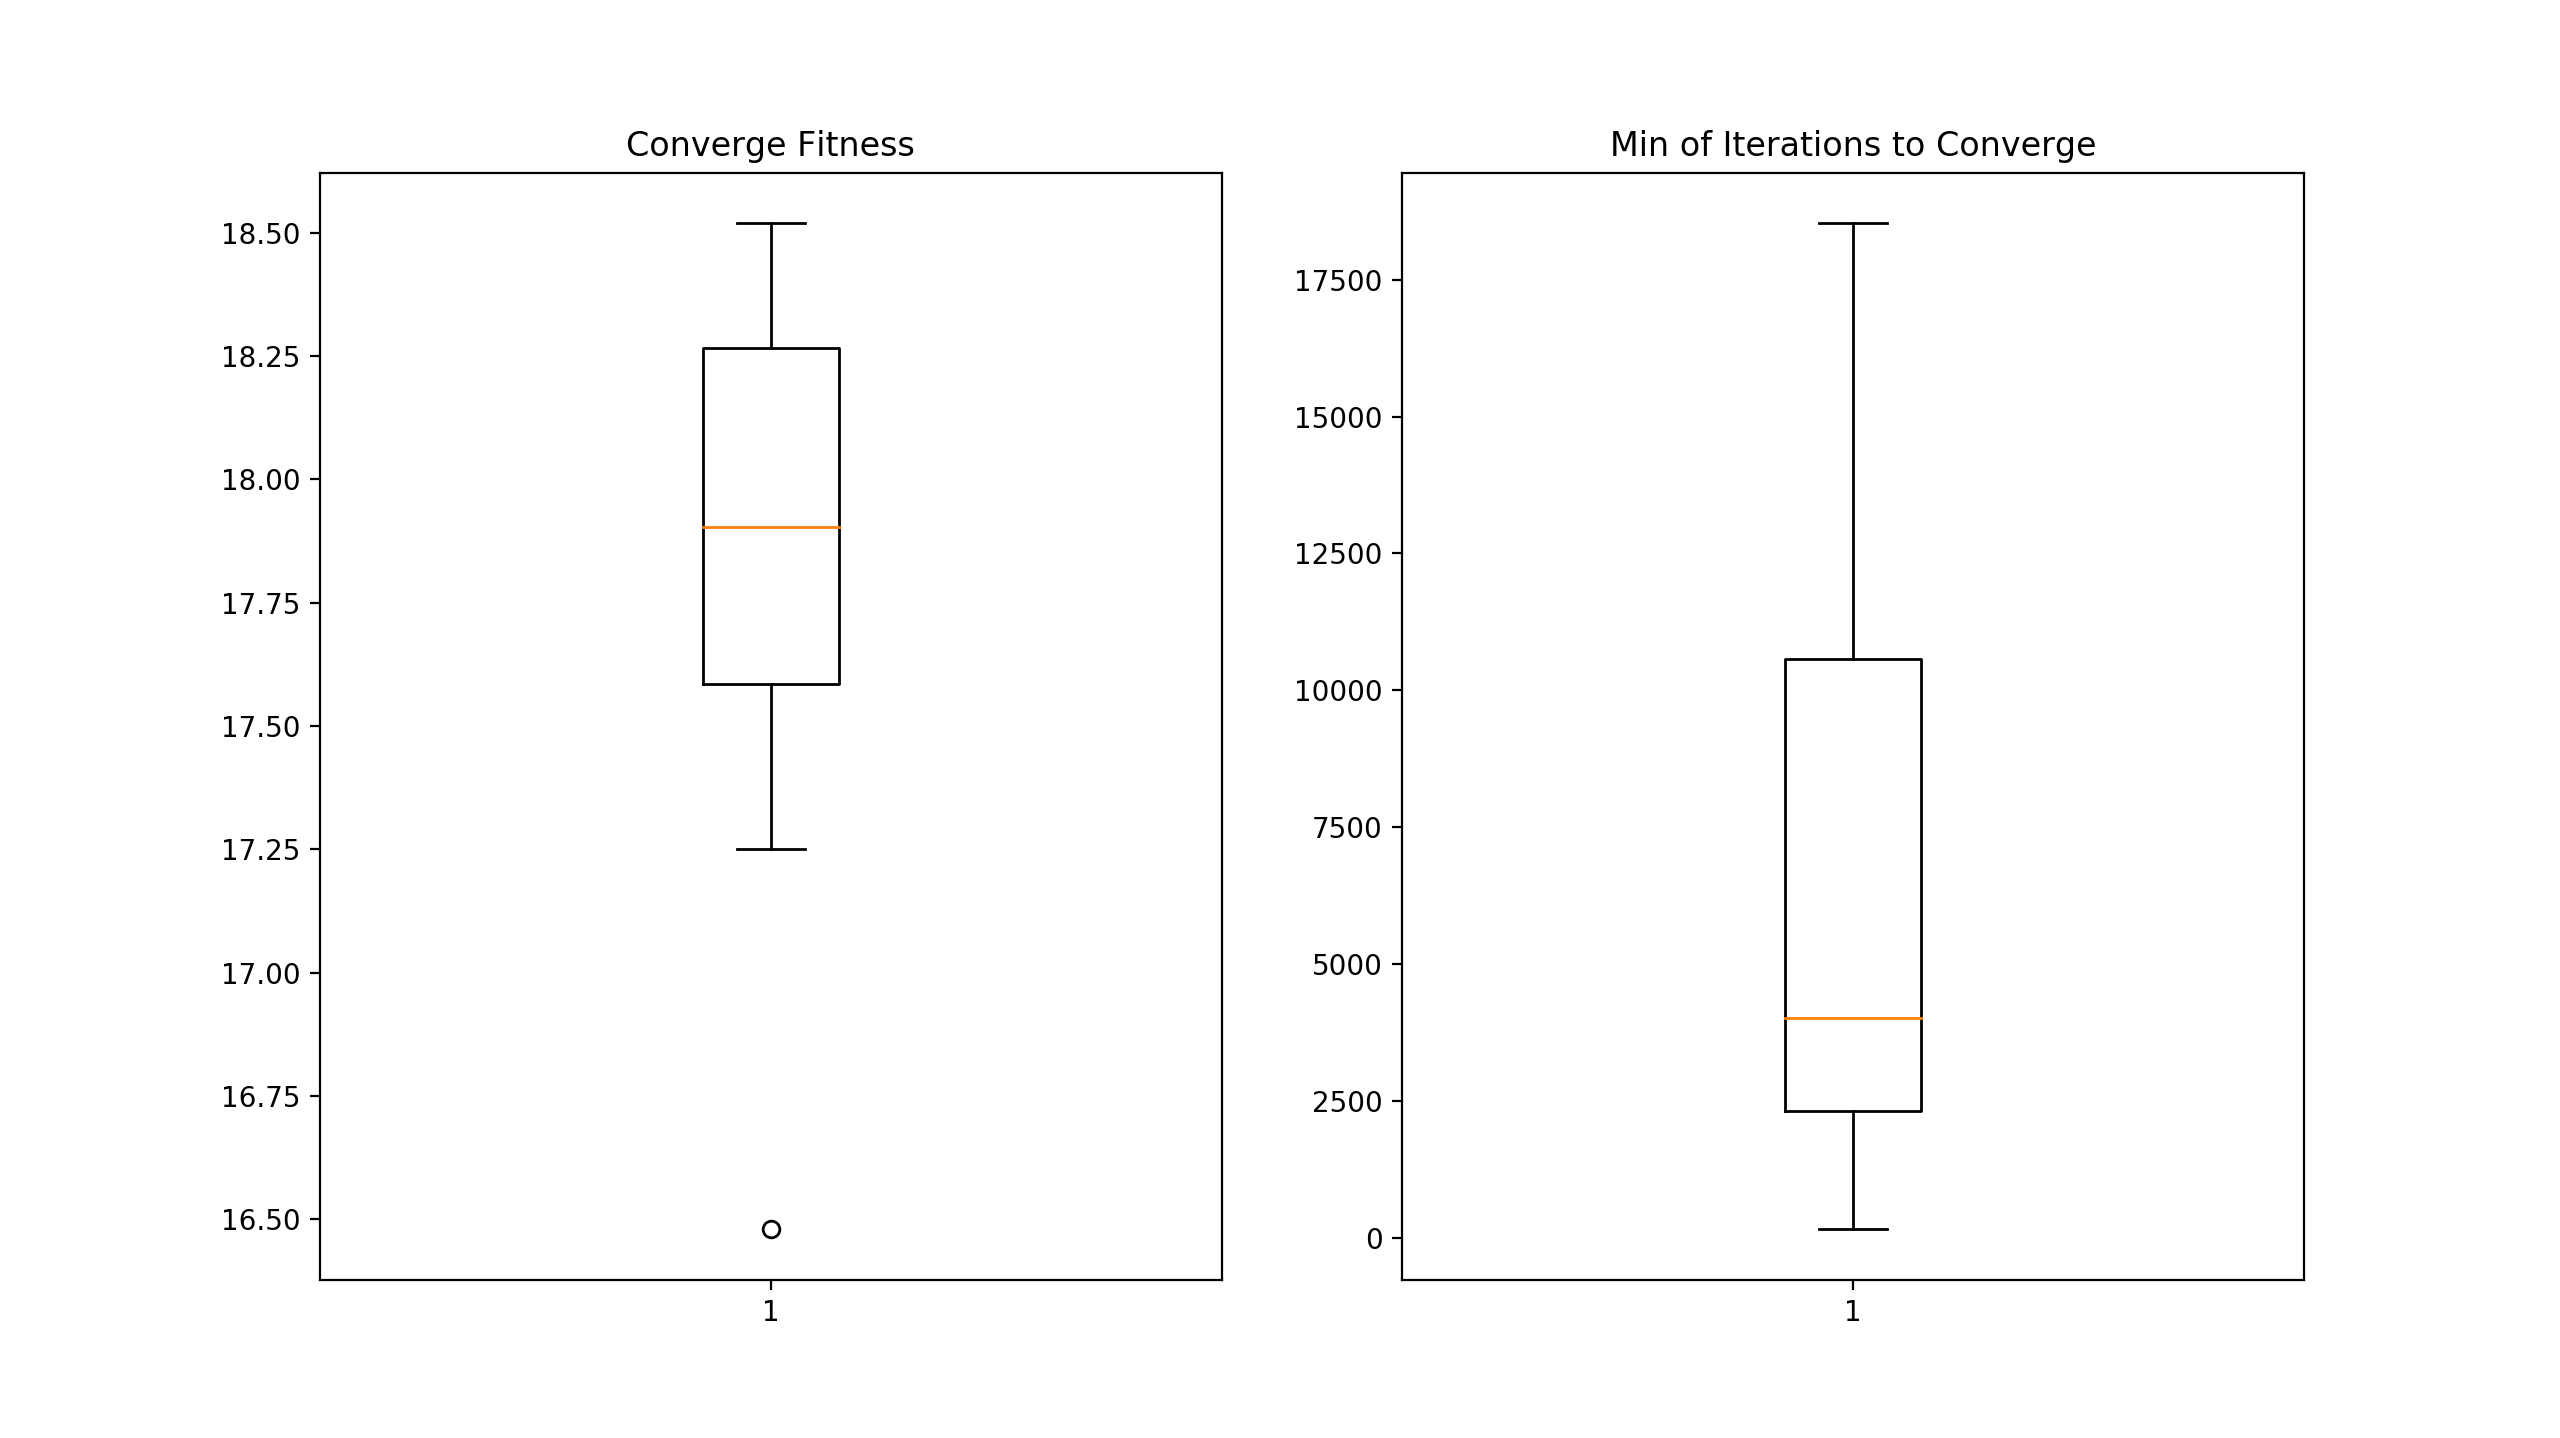
\includegraphics[scale = 0.4]{SimpleEA_gph.png}
    \caption{Boxplot resultado estratégia ingênua}
\end{figure}
\subsection{Segunda abordagem}
Para a segunda estratégia, houve convergência para o mínimo global em todas as tentativas. Tendo uma média de iterações até o ponto de convergência de 5210 e um fitness médio geral de 9.71e-15.
\begin{figure}[h]
    \centering
    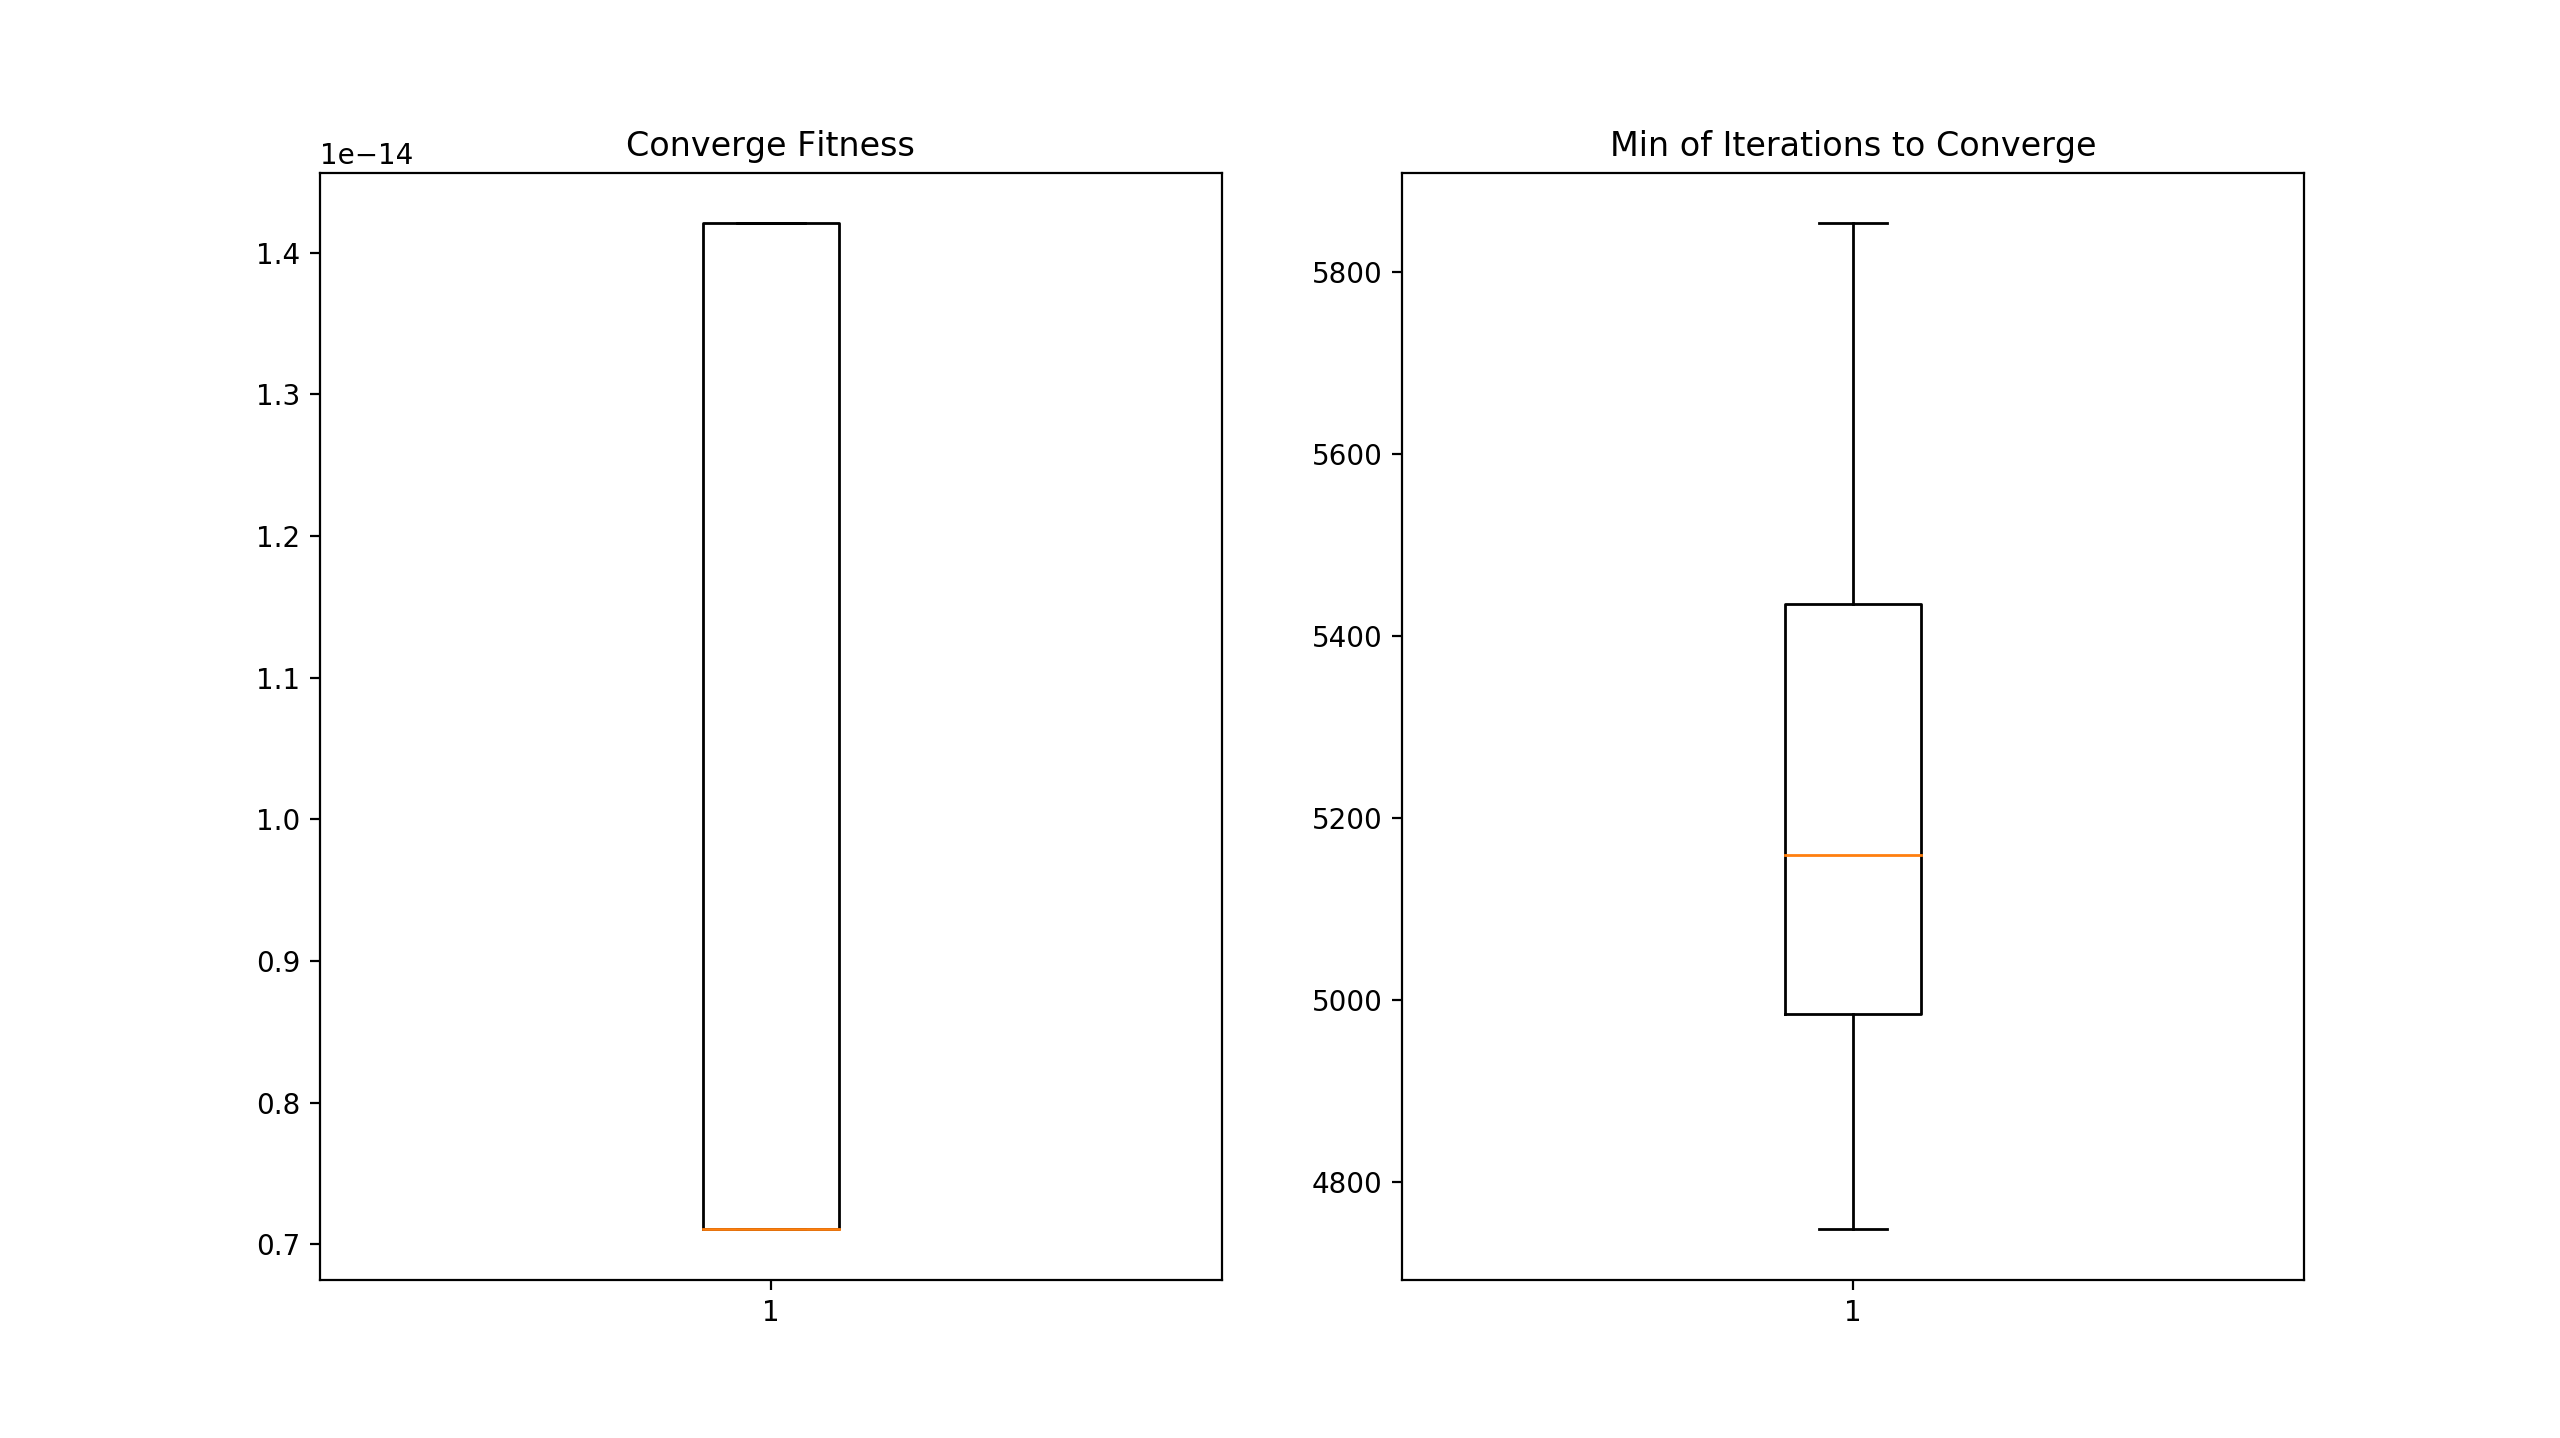
\includegraphics[scale = 0.4]{EA_gph.png}
    \caption{Boxplot resultado segunda estratégia}
\end{figure}
\subsection{Terceira abordagem}
Para a terceira estratégia, houve convergência para o mínimo global em todas as tentativas. Tendo uma média de iterações até o ponto de convergência de 940 e um fitness médio geral de 3.67e-15.
\begin{figure}[h]
    \centering
    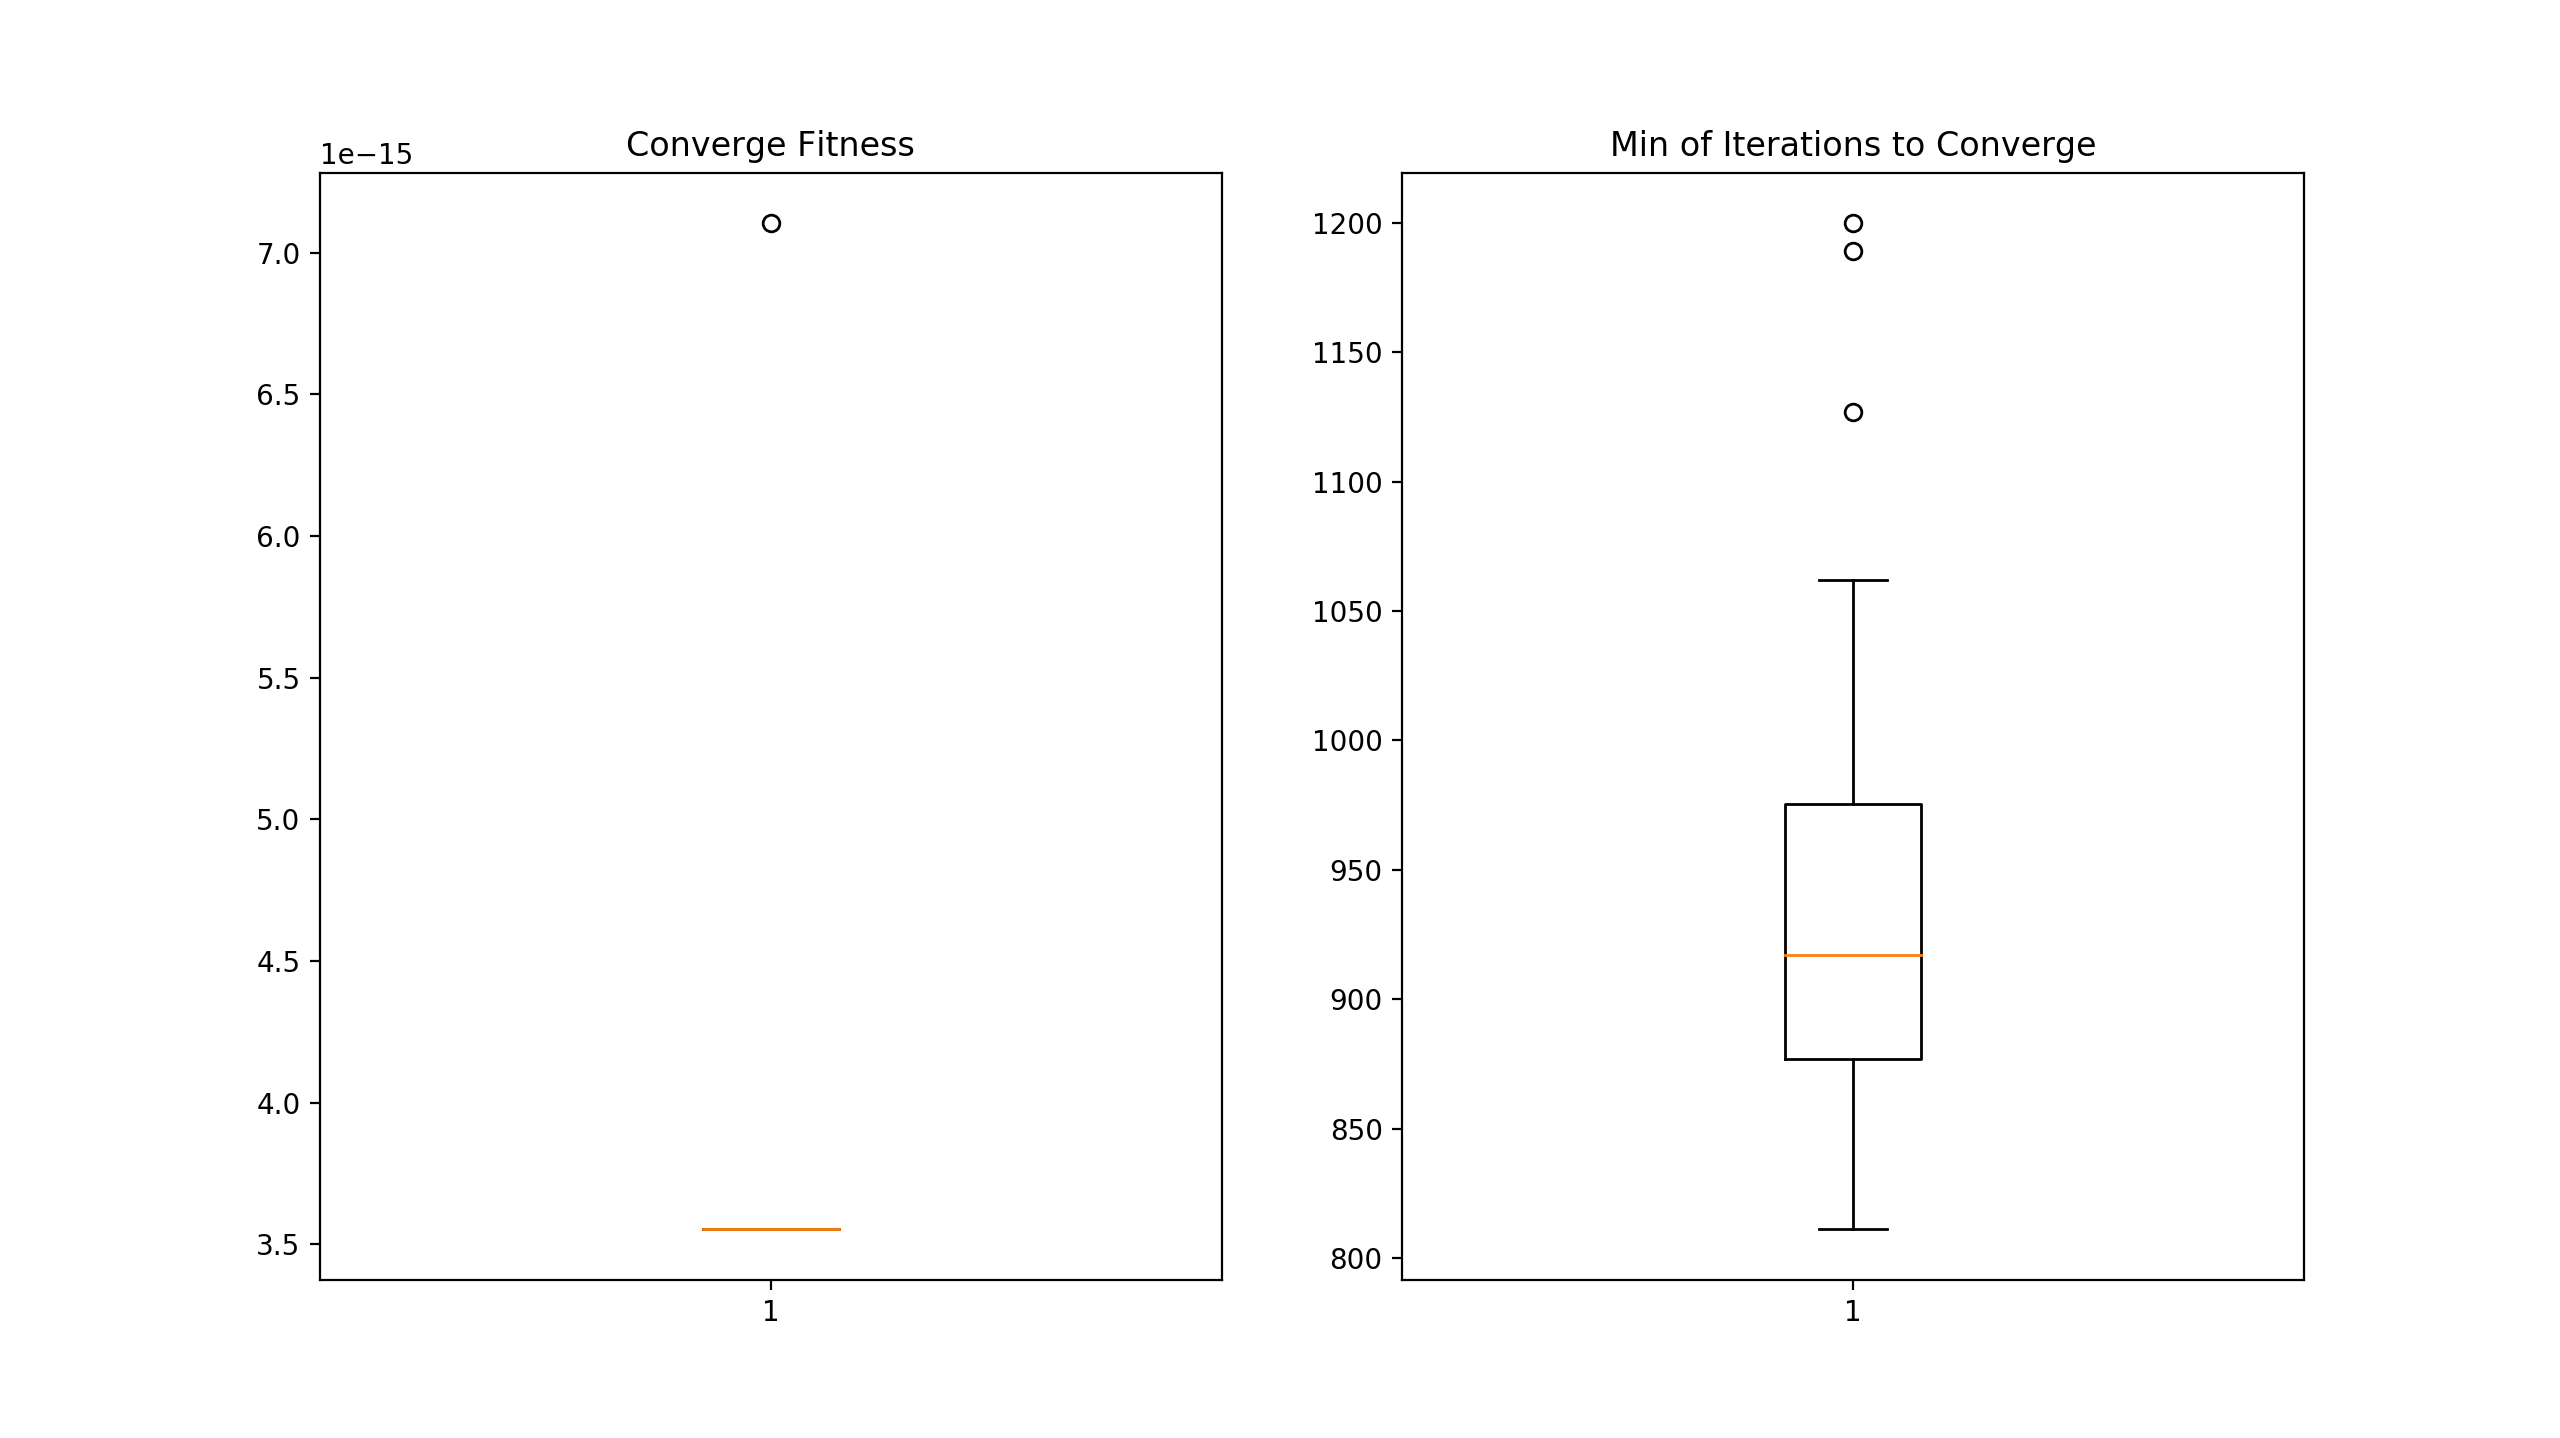
\includegraphics[scale = 0.4]{R_EA_gph.png}
    \caption{Boxplot resultado terceira estratégia}
\end{figure}
% Exemplo de citação
% Consulte o manual da classe \cite{abntex2classe} para uma
% referência completa das macros e ambientes disponíveis.

% Referências
% \bibliography{abntex2-modelo-references}



\end{document}

